% \COMMENT{write a small section for b-spline and imitation learning first}

% \textbf{Problem formulation.} Imitation learning policies $\pi(a \mid o)$ maps observations to actions, where the observation $o$ typically comprises proprioceptive signals (e.g., joint positions/velocities) and visual inputs (e.g., RGB images or depth). A widely used technique is \emph{action chunking}, in which the policy predicts a fixed-length sequence of future actions in a single forward pass. Action chunking encourages temporal consistency and longer-horizon planning~\cite{dp}, and it can mitigate compounding errors during closed-loop execution~\cite{act}.

\section{B-spline Action Representations}

In this section, we formulate the B-spline action representation, which shifts visuomotor control from discrete-time action chunk prediction to continuous and smooth B-spline trajectory generation.

\begin{wrapfigure}{r}{0.48\textwidth}
  \vspace{-15pt}
  \centering
  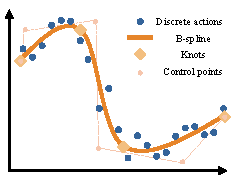
\includegraphics[width=0.5\textwidth]{images/data-fitting-7.pdf}
\caption{\textbf{Adaptive B-spline fitting for demonstration trajectories.}
Given a discrete-time demonstration trajectory, we convert it into a continuous B-spline representation by adaptively selecting knots and estimating control points under a bounded reconstruction error.}
\label{fig:data-fitting}
  \vspace{-20pt}
\end{wrapfigure}

\paragraph{Discrete Action Chunking.} 
We focus on learning a robot policy $\pi(a \mid o)$ from demonstration datasets. The policy maps proprioceptive and visual observations $o_t$ to an \emph{action chunk} 
$\boldsymbol{a}_t = [\boldsymbol a_t,\boldsymbol a_{t+1}, \ldots, \boldsymbol a_{t+T_a}],$
where $T_a$ denotes the prediction horizon.
This action chunking paradigm is widely adopted in modern robot policies~\cite{dp, act, black2024pi_0}, where actions typically correspond to joint positions or end-effector poses.

While predicting action chunks stablizes long-horizon consistency~\cite{dp, block2023provbc, zhang2025actionchunkingexploratorydata}, it also introduces two key limitations for fast manipulation. First, fixed-length chunks impose a uniform temporal resolution across the entire task. Second, independently predicted chunks must be stitched together at inference time, which can create boundary discontinuities that become especially problematic during high-speed execution.

\paragraph{Continuous Action Curves.} To address these limitations, we parameterize the action space as a continuous B-spline trajectory, rather than a discrete sequence of waypoints.


Formally, a B-spline trajectory is defined by a knot vector $U$ and a set of control points $\mathbf{C} = \{c_0, \ldots, c_N\}$. The continuous action at normalized time $u$ is given by
\begin{equation}
    \mathbf{a}(u) = \sum_{i=0}^{N} N_{i,p}(u) \cdot c_i .
\end{equation}
where $N_{i,p}(u)$ is the $i$-th B-spline basis function of degree $p$. In our experiments, we use cubic B-splines, which provide smooth trajectories with continuous velocity and acceleration profiles. This formulation turns the policy output from a fixed list of discrete waypoints into the parameters of a continuous trajectory. The predicted curve can be sampled at any desired control frequency and executed by the low-level controller as a dense stream of commands.


B-splines provide several properties that are particularly useful for fast robot manipulation:
\newline
\textbf{\textit{1) Temporal flexibility}}. Because the action trajectory is defined continuously, the same curve can be sampled at a higher control frequency without changing the policy. This allows the robot to receive dense low-level commands even when the policy runs at a lower inference rate.

\textbf{\textit{2) Temporal rescaling}}. Given a predicted trajectory $\mathbf{a}(u)$, we can execute it faster by scaling the mapping between real time and the curve parameter. For a speedup factor $n$, the robot follows the same action trajectory while traversing the curve more quickly:
$\mathbf{a}_{\mathrm{exec}}(t) = \mathbf{a}(n t)$.
This provides a mechanism for accelerating a learned policy without retraining it for each target execution speed.

\textbf{\textit{3) Intrinsic smoothness}}. B-splines are smooth by construction. Unlike discrete action chunks, which may contain sharp changes between adjacent predictions, a B-spline trajectory produces smooth interpolated actions. This smoothness is especially important under high-speed execution, where abrupt changes in commanded poses can lead to controller tracking errors, overshoot, or task failure.

\textbf{\textit{4) Local error isolation}}. each control point only affects a limited portion of the trajectory. This locality makes the representation stable and compact. Errors in one control point do not globally distort the entire predicted action sequence.


% This formulation provides three critical advantages for robot control: \textbf{(i) Temporal Flexibility:} $a(u)$ can be sampled at arbitrary frequencies or temporally scaled without losing geometric fidelity; \textbf{(ii) Intrinsic Smoothness:} cubic B-splines ($p=3$) guarantee $C^2$ continuity by construction, yielding smooth velocity and acceleration profiles; \textbf{(iii) Local Error Isolation:} the compact support of the basis ensures perturbations in a single control point remain localized, preventing error propagation.
% \begin{itemize}[leftmargin=*]
% \item \textbf{Local Control:} B-spline basis functions have compact support, meaning that perturbations to a single control point affect only a local segment of the trajectory. This property prevents local prediction errors from propagating globally.
% \item \textbf{Smoothness Guarantees:} A B-spline of degree $p$ is inherently $C^{p-1}$ continuous. In this work, we use cubic B-splines ($p=3$), which guarantee $C^2$ continuity and thus ensure smooth velocity and acceleration profiles by construction.
% \item \textbf{Affine Invariance:} Affine transformations applied to the control points induce identical transformations of the resulting curve, making B-splines naturally compatible with standard neural policy architectures.
% \end{itemize}

\begin{figure*}[t]
    \centering
    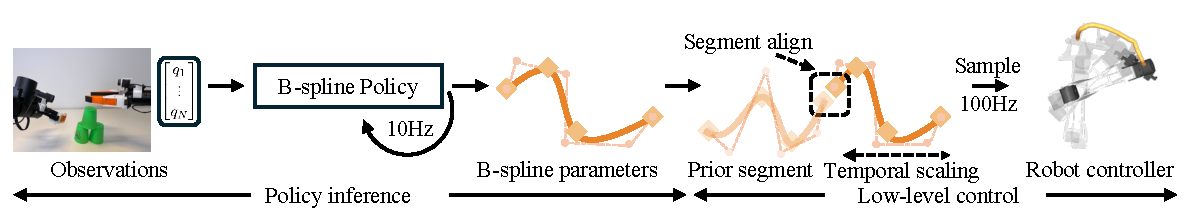
\includegraphics[width=0.98\linewidth]{images/method4.pdf}
    \caption{\textbf{\our inference overview.}
    At each inference step, the policy takes images and proprioception as the input and outputs future B-spline segment parameters.
    %
    At the low-level control stage, we align each successive B-spline segment with the prior one. The predicted B-spline segment can be temporally scaled to adjust execution speed. Actions are then sampled at a higher frequency and sent to the robot controller.}
    \label{fig:method}
    \vspace{-12pt}
\end{figure*}

% This representation naturally supports speedup by scaling real time by a factor of $m$: $a(u) = a(m \cdot t_{\mathrm{real}})$, so the robot executes the trajectory $m$ times faster. Combined with the $C^2$-smooth profile, this reduces overshoot, compounding error, and safety violations~\cite{yin2024offlineimitationlearninggraph} that are critical for maintaining success rates under aggressive speedup. 
%The full procedure is given in Algorithm~\ref{alg:pipeline-inference}.


% However, unlike discrete-time actions, where each action corresponds to a specific timestamp, a B-spline is jointly determined by a knot vector and control points that do not admit a one-to-one alignment in time: knots govern where the basis functions change, while each control point influences a span of the trajectory due to local support.
% As a result, predicting spline parameters raises practical challenges for imitation learning, including how to define fixed-size learning targets when knot spacing is non-uniform and how to handle the additional boundary support required to evaluate a spline segment near its start and end. We detailed how to solve these problems in Sec.~\ref{sec:model-train}.


B-splines offer a natural continuous representation for robot actions, however, using them in a visuomotor policy requires several design choices. In particular, we need to convert discrete demonstrations into B-spline targets, represent non-uniform knots with a fixed-size policy output, and execute consecutive spline segments smoothly. We describe these components in the next section.


\section{B-spline Policy}
\label{sec:model-train}

In this section, we describe how to build a visuomotor policy with B-spline actions and convert discrete demonstrations into fixed-size B-spline targets.

\noindent\textbf{Adaptive B-spline Fitting from Demonstrations.}
% \label{sec:data-preparing}
% 
% 
% 
% 
% 
% 
% 
To train \our, we first convert discrete demonstration trajectories into continuous B-spline trajectories.
%
Given a sequence of demonstration actions, we fit a degree-$p$ B-spline that approximates the original trajectory within an error tolerance. We use an adaptive fitting procedure based on the classical FITPACK strategy~\cite{fitting-bspline,dierckx1995curve,dierckx1982algorithms}, which iteratively inserts knots into trajectory regions with the largest reconstruction error.
\newline
As shown in Fig. \ref{fig:data-fitting}, this adaptive knot placement allocates representation capacity where it is needed most: fewer knots are allocated to smooth regions, while density increases in high-curvature segments. As a result, the fitted B-spline provides a compact continuous representation of the demonstration trajectory while maintaining bounded approximation error, as summarized in Algorithm \ref{alg:spline-compress}.

\begin{wrapfigure}{r}{0.55\textwidth}
\vspace{-20pt}
\centering
\begin{minipage}{0.55\textwidth}
\begin{algorithm}[H]
\caption{Adaptive B-spline Curve Fitting}
\label{alg:spline-compress}
\small
\textbf{Input:} samples $\{(t_i, \mathbf{a}_i)\}_{i=1}^N$, tolerance $\varepsilon$, max knots $|U|_{\max}$ 
\begin{enumerate}[leftmargin=1.2em,itemsep=0pt,topsep=2pt]
\item Initialize $U \gets \{t_1, t_N\}$.
\item \textbf{while} $|U| < |U|_{\max}$:
  \begin{enumerate}[leftmargin=1.2em,itemsep=0pt,topsep=0pt]
  \item Fit degree-$p$ B-spline $\mathbf{a}(\cdot)$ with knots $U$.
  \item $E \gets \max_i \|\mathbf{a}(t_i) - \mathbf{a}_i\|$.
  \item \textbf{if} $E \le \varepsilon$, \textbf{break}.
  \item Insert one knot via FITPACK criterion.
  \end{enumerate}
\item \textbf{return} $U$, $\mathbf{a}(\cdot)$.
\end{enumerate}
\textbf{Output:} knot vector $U$, fitted trajectory $\mathbf{a}(\cdot)$

\end{algorithm}
\end{minipage}
\vspace{-1em}
\end{wrapfigure}


\noindent\textbf{Fixing the Policy Output Size.} After fitting B-splines to the demonstrations, we train a policy to predict B-spline parameters from observations. Directly predicting a full-trajectory spline is inefficient, so the policy outputs the \emph{next} B-spline segment at each step.
\newline
Because B-splines have local support, any trajectory segment can be represented by a fixed number of nearby control points and knots. Unlike discrete action chunks, however, a fixed number of control points does not imply a fixed time horizon because knot intervals may vary. The policy therefore predicts both the control points and knot values, outputting a fixed-size vector of local B-spline parameters, $[U; C]$, that can be used with standard imitation learning architectures with minimal modification.
\newline
In practice, evaluating a degree-$p$ B-spline segment requires neighboring control points and knots for boundary support. We append future control points when available and repeat the final control point near the end of a trajectory, producing fixed-size training targets while preserving valid B-spline evaluation.

% Thanks to the local support of B-splines: each control point affects the trajectory only over a bounded knot span,
% % Leveraging this property, 
% we can parameterize the policy output as fixed-size \emph{segments} containing a constant number of control points.
% However, because our knot vectors are generally non-uniform, a fixed number of control points does not map to a fixed temporal horizon, each \emph{B-spline segment} represents a trajectory segment with variable temporal length. To accommodate this non-uniformity without complex architectural changes,
% %This non-uniformity further implies that the knots associated with each segment must also be predicted.
% we treat knot values as additional action dimensions and jointly predict control points and knots.
% This allows us to directly reuse standard imitation learning architectures without architectural modifications.



% \begin{figure}[t] % 双栏论文用 figure*；单栏可以改成 figure
% \centering

% \begin{minipage}[t]{0.45\textwidth}
% \begin{sidealgorithm}{Adaptive B-spline Fitting}{alg:spline-compress}

% \textbf{Input:} samples $\{(t_i, \mathbf{a}_i)\}_{i=1}^N$, tolerance $\varepsilon$, maximum knot count $|U|_{\max}$ \\
% \textbf{Output:} knot vector $U$ and fitted trajectory $\mathbf{a}(\cdot)$

% \begin{enumerate}[leftmargin=1.2em,itemsep=0.25em]
% \item Initialize $U \gets \{t_1, t_N\}$.
% \item \textbf{while} $|U| < |U|_{\max}$:
%   \begin{enumerate}[leftmargin=1.2em,itemsep=0.15em]
%   \item Fit a degree-$p$ B-spline trajectory $\mathbf{a}(\cdot)$ using knots $U$.
%   \item Compute $E \gets \max_i \|\mathbf{a}(t_i) - \mathbf{a}_i\|$.
%   \item \textbf{if} $E \le \varepsilon$, \textbf{break}. \hfill\textit{(early stop)}
%   \item Insert one knot into $U$ using the FITPACK knot-insertion criterion.
%   \end{enumerate}
% \item \textbf{return} $U$ and $\mathbf{a}(\cdot)$.
% \end{enumerate}

% \end{sidealgorithm}
% \end{minipage}
% \hfill
% \begin{minipage}[t]{0.53\textwidth}
% \begin{sidealgorithm}{Inference pipeline}{alg:pipeline-inference}

% \textbf{Input:} policy $\pi$, speedup factor $m$, inference budget $\delta^{\text{budget}}$ \\
% \textbf{State:} current B-spline segment $S$, segment start time $t_0$, in-flight inference flag in\_flight

% \begin{enumerate}[leftmargin=1.2em,itemsep=0.25em]
% \item \textbf{Initialize:} $S \leftarrow \pi(o_{\text{recent}})$,\quad $t_0 \leftarrow \text{now}()$,\quad in\_flight $\leftarrow$ false.
% \item \textbf{Loop (control at high rate):}
% \begin{enumerate}[leftmargin=1.2em,itemsep=0.15em]
% \item $t_{\text{real}} \leftarrow \text{now}() - t_0$, \quad $u \leftarrow m \cdot t_{\text{real}}$ \hfill\textit{(Speedup)}
% \item Execute $a \leftarrow S(u)$ \hfill\textit{(Sample)}
% \item \textbf{If} $(u_{\max}(S) - u) < \delta^{\text{budget}}$ and in\_flight = false:
% \begin{enumerate}[leftmargin=1.2em,itemsep=0.1em]
% \item Launch asynchronous inference to obtain a new segment $S_{\text{new}} \leftarrow \pi(o_{\text{recent}})$
% \item Set in\_flight $\leftarrow$ true
% \end{enumerate}
% \item \textbf{On inference completion:} let $T^{\text{inf}}$ be the measured inference latency.
% \begin{enumerate}[leftmargin=1.2em,itemsep=0.1em]
% \item Compute alignment time $t^\star$ by Eq.~\eqref{eq:align-time} using $S_{\text{new}}$ and $a_{\text{last}}$
% \item Swap $S \leftarrow S_{\text{new}}$
% \item Update $t_0 \leftarrow \text{now}() - \frac{t^\star}{m}$ \hfill\textit{(Segment align)}
% \item Set in\_flight $\leftarrow$ false
% \end{enumerate}
% \end{enumerate}
% \end{enumerate}

% \end{sidealgorithm}
% \end{minipage}
% \end{figure}






% Due to the local support of B-spline basis functions, evaluating a degree-$p$ B-spline segment over an interval $[t_i, t_j]$ with $j > i$ depends not only on the control points within the interval, but also on neighboring knots and control points.
% Specifically, the segment requires the knot sequence
% \(t_{i-p}, \ldots, t_j, \ldots, t_{j+p}\)
% and the corresponding control points
% \(c_{i-p}, c_{i-p+1}, \ldots, c_{j-1}\).
% In other words, a segment spanning $(j-i)$ knot intervals uses $N_c = (j-i)+p$ control points and requires $N_c + p + 1$ knots.
% To ensure consistent input dimensionality across segments, we extend the control-point sequence as follows:
% a) For segments at the beginning of a trajectory or in the middle, we append the subsequent control points $c_j, \ldots, c_{j+k}$ to provide the necessary forward support.
% b) For segments at the end of a trajectory, where future control points are unavailable, we repeat the final control point to supply the missing support and align the required numbers of control points and knots.
% Overall, this design requires only minimal changes to existing imitation-learning pipelines. 

% The policy is supervised on knot vectors from spline fitting and predicts knots jointly with control points $[t;c]$; predicted knots almost always remain monotonic, and the rare violations near trajectory ends are corrected by a lightweight projection detailed in the appendix.

% \subsection{Smooth and Fast Execution.}


% \noindent\textbf{Fast Real-Time Execution.}
% \label{sec:inference}

\paragraph{High-frequency Execution and Temporal Rescaling.}
During inference, we decouple the policy inference rate from the low-level control rate. The visuomotor policy runs at a relatively low frequency and predicts a future B-spline segment. The low-level controller then samples this continuous segment at a much higher frequency to generate dense robot commands.

This design is important for fast manipulation. When executing a policy faster than the demonstration, discrete action chunks may become too sparse or discontinuous for reliable tracking. In contrast, a B-spline segment can be sampled densely after temporal rescaling, allowing the controller to receive smooth high-frequency commands even when the policy itself runs at a lower rate.

Because the predicted trajectory is continuous, we can directly adjust its execution speed by changing the mapping between real time and the spline parameter. Given a predicted trajectory $\mathbf{a}(u)$ and a target speedup factor $n$, the executed action is $\mathbf{a}_{\mathrm{exec}}(t) = \mathbf{a}(nt)$. This preserves the geometric shape of the predicted action trajectory while traversing it faster in real time.

% \noindent\textbf{High-Frequency Inference.}
% To ensure that time-critical control commands are issued reliably, especially under aggressive speedup, we decouple the policy inference rate from the low-level control rate during execution, as illustrated in Fig.~\ref{fig:method}.
% The policy operates at a lower frequency to predict a future B-spline parameter segment, while the low-level controller samples actions from the resulting continuous trajectory at a much higher frequency. This design preserves dense command updates under temporal scaling, enabling reliable tracking and precise manipulation at high execution speeds.
% % This decoupling allows the system to issue time-critical control commands at high rates during fast or dynamic motions without increasing the computational cost of policy inference.



\noindent\textbf{Pipelined Execution with Segment Alignment.}
For long-horizon tasks, the policy repeatedly predicts new B-spline segments while the robot is executing the previous one. A naive pipelined implementation assumes that the beginning of the newly predicted segment aligns with the unexecuted tail of the previous segment. In practice, this assumption is often violated due to policy prediction noise, inference latency, and controller tracking error. As a result, directly switching to the new segment can introduce discontinuities at segment boundaries.

To address this issue, we introduce an inference-time segment alignment mechanism. Let $a_{\text{last}}$ denote the most recently executed action, and let $S{\mathrm{new}}(t)$ denote the newly predicted B-spline segment evaluated at relative time $t$. Instead of starting the new segment at a fixed time determined only by inference latency, we search for the point on the new segment that best matches the current executed action:
\begin{equation}
\label{eq:align-time}
t^\star = \arg\min_{0 \leq t \leq \lambda T_{\mathrm{inf}}}
\mathrm{MSE}\big(S_{\mathrm{new}}(t), a_{\text{last}}\big),
\end{equation}

where $T^{\text{inf}}$ is the measured inference latency and $\lambda > 1$ slightly enlarges the search window for robustness. The controller then begins executing the new segment from $t^\star$.

This alignment step reduces boundary mismatch between consecutive B-spline segments and prevents small discontinuities from accumulating over time. As shown in our experiments, this becomes especially important under high-speed execution, where even small jumps in commanded actions can lead to tracking errors or task failure.

% \noindent\textbf{Pipelined Execution with Segment Alignment.}
% To maximize throughput and amortize inference latency, we adopt a pipelined execution strategy.
% Naively applying asynchronous inference assumes that the beginning of a newly predicted trajectory coincides exactly with the unexecuted tail of the previous trajectory.
% Under this assumption, the new trajectory is evaluated at the current time, and the portion corresponding to the inference latency is discarded.
% %
% In practice, prediction noise and execution delays frequently violate this assumption, resulting in discontinuities at segment boundaries.
% As execution speed increases, these discontinuities become the dominant failure mode, leading to compounding tracking errors, increased retries, and reduced overall throughput.
% Crucially, because our policy outputs an explicit continuous trajectory via a B-spline parameterization, we can directly address this mismatch.
% We introduce an inference-time \emph{segment alignment} mechanism that selects a more suitable starting point within the initial segment of the newly predicted trajectory.
% Let $a_{\text{last}}$ denote the most recently executed action, and let $T^{\text{inf}}$ be the measured inference latency.
% Let $S_\text{new}(t)$ denote the action evaluated at relative time $t$ along the newly predicted trajectory.
% We determine the alignment time by solving
% % \begin{equation}
% % \label{eq:align-time}
% % t^\star
% % = \arg\min_{0 \le t \le \lambda T^{\text{inf}}}
% %     \operatorname{MSE}\!\left(S_{\text{new}}(t),\, a_{\text{last}}\right),
% % \end{equation}
% $t^\star = \arg\min_{0 \le t \le \lambda T^{\text{inf}}} \operatorname{MSE}\!\left(S_{\text{new}}(t),\, a_{\text{last}}\right)$
% where $\lambda > 1$ (chosen close to $1$) slightly extends the search window beyond the nominal inference latency to improve robustness.
% This alignment reduces boundary discontinuities and prevents compounding tracking drift, which is essential for maintaining stable performance at high execution speeds.

% \begin{algorithm}[t]
% \setlength{\intextsep}{0pt}
% \setlength{\columnsep}{6pt}
% \begin{wrapfloat}{algorithm}[24]{r}{0.5\textwidth}
% \caption{Inference pipeline}
% \label{alg:pipeline-inference}
% \textbf{Input:} policy $\pi$, speedup factor $m$, inference budget $\delta^{\text{budget}}$ \\
% \textbf{State:} current B-spline segment $S$, segment start time $t_0$, in-flight inference flag \quad in\_flight
% \begin{enumerate}[leftmargin=1.2em]
% \item \textbf{Initialize:} $S \leftarrow \pi(o_{\text{recent}})$,\quad $t_0 \leftarrow \text{now}()$,\quad in\_flight $\leftarrow$ false.
% \item \textbf{Loop (control at high rate):}
% \begin{enumerate}[leftmargin=1.2em]
% \item $t_{\text{real}} \leftarrow \text{now}() - t_0$, \quad $u \leftarrow m \cdot t_{\text{real}}$ \hfill(\textit{Speedup})
% \item Execute $a \leftarrow S(u)$ \hfill(\textit{Sample})
% \item \textbf{If} $(u_{\max}(S) - u) < \delta^{\text{budget}}$ and in\_flight = false:
% \begin{enumerate}[leftmargin=1.2em]
% \item Launch asynchronous inference to obtain a new segment $S_{\text{new}} \leftarrow \pi(o_{\text{recent}})$
% \item Set in\_flight $\leftarrow$ true
% \end{enumerate}
% \item \textbf{On inference completion:} let $T^{\text{inf}}$ be the measured inference latency.
% \begin{enumerate}[leftmargin=1.2em]
% \item Compute alignment time $t^\star$ by Eq.~\eqref{eq:align-time} (using $S_{\text{new}}$ and $a_{\text{last}}$)
% \item Swap $S \leftarrow S_{\text{new}}$
% \item Update $t_0 \leftarrow \text{now}() - \frac{t^\star}{m}$ \hfill(\textit{Segment align})
% \item Set in\_flight $\leftarrow$ false
% \end{enumerate}
% \end{enumerate}
% \end{enumerate}
% \end{wrapfloat}
% \end{algorithm}

% The complete procedure is provided in detail in Algorithm~\ref{alg:pipeline-inference} in the appendix.


% \noindent\textit{PD control with feedforward terms.}
% To preserve tracking accuracy under retiming and fast execution, we employ a PD controller augmented with model-based feedforward terms~\cite{santibanez2001pd,sciaviccomodeling,grotjahn2002model}:
% \begin{equation}
% \label{eq:ff}
% \boldsymbol{\tau} = \underbrace{\boldsymbol{K}_p(\boldsymbol{q}_d - \boldsymbol{q}) + \boldsymbol{K}_d(\dot{\boldsymbol{q}}_d - \dot{\boldsymbol{q}})}_{\text{PD}} + \underbrace{\boldsymbol{M}(\boldsymbol{q}_d)\ddot{\boldsymbol{q}}_d + \boldsymbol{C}(\boldsymbol{q}_d,\dot{\boldsymbol{q}}_d)\dot{\boldsymbol{q}}_d + \boldsymbol{g}(\boldsymbol{q}_d)}_{\text{feedforward}},
% \end{equation}
% where $\boldsymbol{q}_d, \dot{\boldsymbol{q}}_d, \ddot{\boldsymbol{q}}_d$ are the desired joint states obtained analytically from B-spline derivatives, avoiding numerical-differentiation noise at high speeds. Symbol definitions and gain values are detailed in the appendix.

% Because the trajectory is parameterized as a continuous spline, desired velocities and accelerations can be efficiently obtained at arbitrary time instances by evaluating spline derivatives, enabling accurate feedforward control without numerical differentiation.

% Besides, we employ a pipelined execution strategy to prevent the robot
% from idling while waiting for model predictions. The existing pipeline as in~\cite{}
% implicitly assumes that the initial portion of the newly predicted trajectory
% exactly matches the unexecuted tail of the previous trajectory. Under this
% assumption, the pipeline simply restarts each new chunk at the current time,
% discarding the portion of the predicted trajectory corresponding to the inference
% latency. In practice, this assumption doesn't always hold and introduces
% noticeable discontinuities between consecutive chunks. Now that we have an exact
% parametric representation of the predicted trajectory, we can directly address
% this mismatch.

% We introduce an inference-time alignment mechanism that selects a more suitable
% starting point within the initial segment of the newly predicted trajectory.
% Let $a_{\text{last}}$ denote the most recently executed action, and let
% $T^{\text{inf}}$ be the actual model inference latency. Because the new
% trajectory is represented as a continuous B-spline parameterization, the
% predicted action at relative time $t$ in the new chunk is denoted by
% $\mathrm{NewChunk}(t)$. We determine the alignment point by solving this problem:
% \begin{equation}
% \label{eq:align-time}
% t^\star
% = \arg\min_{0 \le t \le \lambda T^{\text{inf}}}
%     \operatorname{MSE}\!\left(\mathrm{NewChunk}(t),\, a_{\text{last}}\right),
% \end{equation}
% where the search range is slightly extended by a factor $\lambda>1$ (but close to
% 1) to allow matching against points just beyond the exact inference window. This
% extension improves robustness empirically. The detailed algorithm is shown in the supplementary meterials.

% Besides the PD-controller used in many existing works~\cite{}, we also implement a PD-controller with feedforward control~\cite{santibanez2001pd,sciaviccomodeling,grotjahn2002model} to help tracking. This is an additional advantage of \our, as we can get the velocities and the acceleration at any time of the trajectories just by calculating the derivatives of the B-splines.
